%fitts law in use (methods)
\section{Fitts' Law} \label{sec:M:fittsLaw}

%present how the fitts gui works
%subject reaches target
%variables for the performance metrics are recorded 
%performance metrics are calculated (but are first presented in results)

As stated in \secref{sec:BG:validatingPerformance} on the theory behind Fitts Law, this project will utilize a modified Fitts' Law task consisting of a virtual target reaching test to evaluate the progress of subjects going through user training. Additionally the proposed additional performance metrics, throughput, path efficiency, overshoot, stopping distance and completion rate will be used in this project. The following section describes how the Fitts' Law task has been implemented in this project.

\subsection{Virtual target reaching test} \label{sub:M:targetReachingTest}

The virtual targets reaching test is implemented into the same GUI used for data acquisition and user training, first mentioned in \secref{sec:M:dataAcquisition}. Different functions have been build into the GUI to enable switching between different usages by the press of a button. When switching to the function of the target reaching test the subject is met with the interface shown in \figref{fig:fittsLawTask}. Here the subjects control the position of the cursor by performing movements shown by the borders of the grid area. Thus, extension of the hand will move the cursor to the right of the grid, and flexion will move the cursor to the left. Similarly, radial and ulnar deviation moves the cursor up and down respectively. This approach is used to improve the intuitiveness of the control where the direction of the cursor relate to the directions subjects will perform movements of the hand to control the cursor, when placed as instructed in the protocol, \appref{sec:protocol:experiment} \fxnote{appref virker måske bedre en en secref til protokollen når vi får bygget en ordentlig main med et rigtigt appedix så protokollerne heller ikke står under bibliografien}
Subjects can control the size of the cursors red area by opening and closing the hand, where an open hand will increase the area and a closed hand will decrease the area. Each target is presented by an area with a center and an outer circle. Targets exist in to sizes to facilitate use of the index of difficulty for the throughput metric. The target reaching test consists of reaching a total of 16 targets which each appear for 15 seconds at positions around the center of the grid area. The order of appearance is fixed for each trial but the same across subjects, thus individual subjects will experience the targets as appearing in a new order with each trial. 

\begin{figure}[H] 
	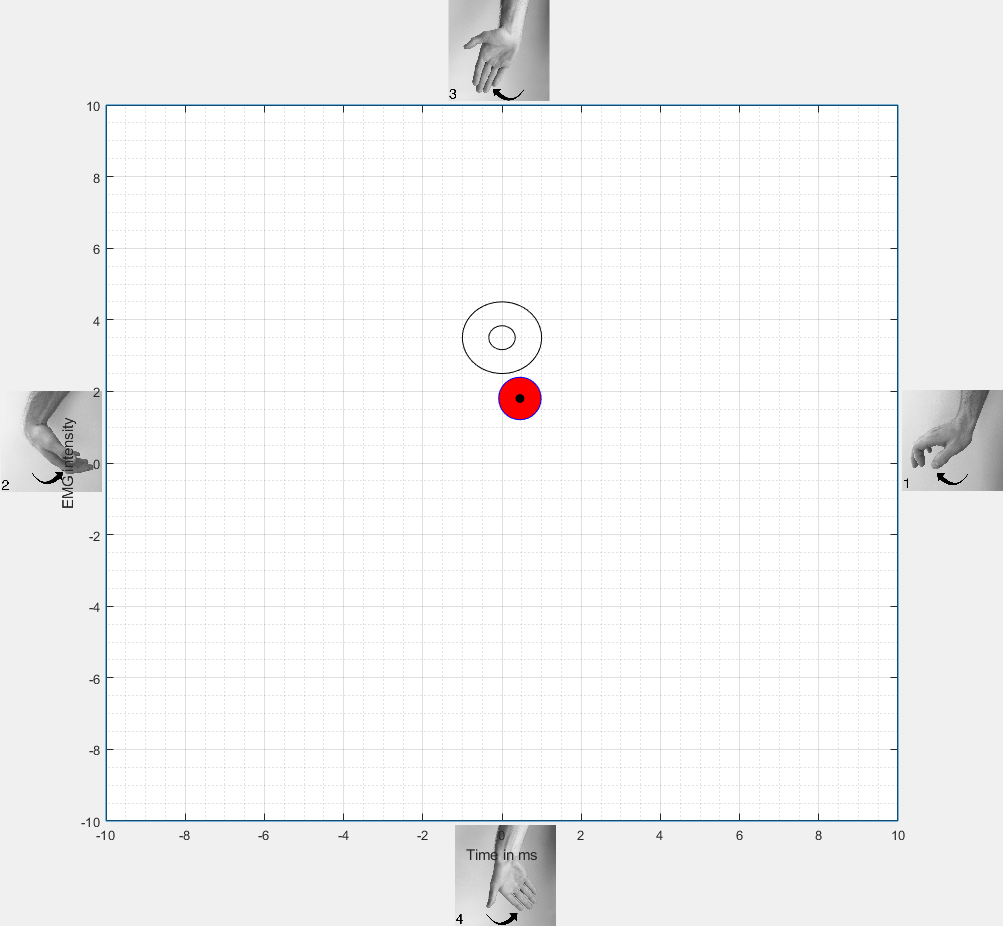
\includegraphics[width=1\textwidth]{figures/xBackground/perftestGUI}
	\caption{The implemented interface for the Fitts' Law task. The grid is the area in which the subject must reach targets with the controlled cursor. The cursor is the red circle area with the black dot in the center. Targets are shown as a circle area with an outer bigger circle. At each border of the grid area a hand movement tis shown. Performing shown movement will move the cursor in the direction of the picture.}
	\label{fig:fittsLawTask}
\end{figure}

Subject must reach the targets inner circle with the cursor dot and expand or decrease the red area of the cursor to reach a size close to that of the target. A moderate size threshold have been implemented to make it possible to reach targets, without a 100\% accuracy of control. If a subject reach a target, the cursor will change color from red to blue, and a bell chime will sound to indicate that the target was reached. The cursor position will be reset to the center of the grid area and the color of the cursor will revert back to red when a new target appears. If a target is not reached within 15 seconds the current target will disappear, a new target will show and the cursor position will be set to the center of the grid area. The approach of resetting the cursor position after each target is to equalize the path for every subject. 

Behind the scene of the target reaching test several metrics are recorded. A trace of the cursor movement throughout the whole test is recorded to decide the subjects path deviation from the optimal path to calculate the path efficiency and distances to targets, stated in \secref{sub:BG:fitts}. An example of a cursor trace is shown in \figref{fig:cursorTrace}. 

\begin{figure}[H] 
	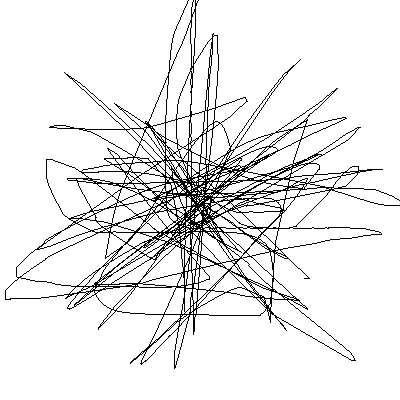
\includegraphics[width=1\textwidth]{figures/pMethods/cursorTrace}
	\caption{The trace of the cursor movement after a target reaching test. This information is not visible or shown to subjects.}
	\label{fig:cursorTrace}
\end{figure}

The number of times a target is reached and exited without completing the dwell time, is recorded and used to calculate subjects overshoot, as stated in \secref{sub:BG:fitts}. Similarly to tracking the travelled distance of the cursor inside the grid area, the travelled distance inside of each target is also recorded to calculate the stopping distance. The number or reached targets is recorded. The total time used to complete the task of reaching the 16 targets is know as $16 ~targets~*~15s = 240s = 4~min$. 

Following the completion of recording target reaching test data from all subjects the performance metrics introduced in \secref{sec:BG:fitts} are calculated and presented in the Results: \chapref{chap:Results}.




